\section{Przechowywanie i transmisja danych}
\label{sec:przesyl}

\subsection{GIS}
\label{subsec:gis}

GIS(Geographical Information Systems) jest to System Informacji Geograficznych, jest to zbiór wiedzy, informacji do pozyskiwania i analizowania danych przestrzennych. Dane są pobieranie w trakcie naziemnych pomiarów jak i zbierane przy użyciu systemu GPS. Informacje te są następnie zapisywane do określonych formatów,dzięki czemu możliwa jest ich dalsza analiza. \underline{\texttt{http://www.gis-support.pl/co-to-jest-gis/}}

\subsubsection{Wykorzystywany układ współrzędnych}
\label{subsec:uklad}

Istnieje wiele układów współrzędnych któe służą do opisu pojedyńczego punktu na powierzchni ziemi.Na stronie \underline{\texttt{http://www.spatialreference.org/ref/epsg/}} (dostęp 20.08.2013) znajduje się lista zawierająca przykłady zapisu punktu na kuli ziemskiej przy użyciu różnych formatów, zawierają one niezbędne infomacje do poprawnego zapisu danych w określonym formacie.

Tradycyjny zapis oparty jest na wykorzystaniu stopni, minut i sekunk, jest on obecnie wypierany przez nowszy,łatwiejszy do obliczeń komputerówych. Wersją która ma za zadanie być ogólnoświatowym formatem jest WGS(World Geodetic System). Jego ostatnia wersja  WSG84 jest powszechnie używana w urządzeniach do nawigacji. Poniżej zaprezentowano jak wygląda zapis w starszym i nowszym punktu określającego położenie budynku A-0 uczelni AGH.

\begin{itemize}

\item
Pierwotny zapis

50°03'52.2803", 019°55'23.7968"
\item
Zapis unowocześniony

50.06452231874906, 19.923276901245117
\end{itemize}

Drugi zapis został wykorzystany do przechowywania danych w plikach, tak aby wymiana i wspólna praca była jak najprostsza. Wybór ten sprawił że nie występuje problem konwersji punktu do formatu czytelnego dla komputera, można go bez problemu odczaytać jako liczbę.

\subsection{Format zapisu}
\label{subsec:zapisWektorowy}

W celu przechowywania obiektu graficznych zdecydowano się na wykorzystanie grafiki wektorowerj.  Oprócz bez problemowej skalowalności, pozwala on również na szeroką i łatwą edycję. W prosty sposób można dodać informacje nie tylko o położeniu, ale inne takie jak słowny opis miejsca lub wydarzenia które miało miejsce w pobliskim rejonie.
Obraz jest w tym przypadku przechowywany jako zbiór formuł matematycznych m.in. proste i łuki. Dzięki takiemu podejściu obraz w dowolnej skali na identyczną jakość, widać to na rysunku \ref{fig:wekt}. Przykładowymi formatami są GML(Geography Markup Language) otwarty standart XML dla wymiany danych GIS, Shapefile czy tradycyjny kartezjański układ współrzędnych.

  \begin{figure}[H]
  \centering
    
\includegraphics[width=50mm]{ge/a1.jpg}
  \caption{Zapis wektorowy}
  \label{fig:wekt}
  \end{figure}

Przeciwnym podejściem jest grafika rastrowa, jest to zapis punktów o określonym kolorze i położeniu na płaszczyźnie. Efektem takiego podejścia jest pogorszenie obrazu w momencie dużego powiększenia. Przykładem są formaty takie jak ADRG,ASC czy RGB.
Porównanie litery a i jej 7-krotnego powiększenia w tym zapise zaprezentowano na rysunku \ref{fig:rast}
  \begin{figure}[H]
  \centering
    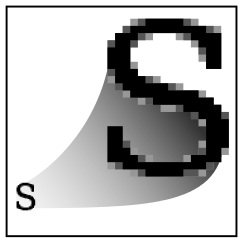
\includegraphics[width=50mm]{ge/a2.jpg}
  \caption{Zapis rastrowy}
  \label{fig:rast}
  \end{figure}

\subsection{Format pliku}
\label{subsec:fileformat}

W celu wypełnienia założeń projektu jakim jest umożliwienie przechowywania danych w zewnętrznym pliku przeprowadzono analizę dostępnych foramtów zapisu danych kartograficznych.

\begin{itemize}

\item
SWDE(Standard Wymiany Danych Ewidencyjnych) - polski format służący głównie do wymiany danych ewidencyjnych gruntów i budynków

\item
SWING(Standard Wymiany INformacji Geodezyjnych) - format danych geodezyjnych służący do wymiany danych pomiędzy bazami danych systemów informatycznych SIT(wikipedia.pl)

\item
KML(Keyhole Markup Language) - otwarty standart oparty na XML-u, stworzony głównie dla potrzeb GoogleEarth

\item
GML(Geography Markup Language) - stworzony przez OGC(Open Geospatial Consortium),międzynarodową organizację założoną w celu tworzenia i rozpowszechniania standarów związanych z informacjami dotyczących geograficznych i geoprzestrzennych danych

\end{itemize}

Dwa polskie formaty są stosunkowo mało popularne, są one głównie wykorzystywane w celu kompunikacji pomiędzy rządowymi bazami danych. Zawierają one bardzo określone typy danych co sprawia że są mało przydatne dla omawianego projetku. KML jest foramtem który posiada szeroki wachlarz dostępnych znaczników a jego duża popularność dostarcza dużą bazę plików gotowych do wykorzystania. Niestety został on stworzony by współpracować z określonym programem, zaimplementowane zostały jedynie elementy które mogą zostać wykorzystane w nim. Ostani przykład został stworzony w uniwersalnym celu do ogólnego użytku, posiada on bardzo dużo możliwości, apadtacji do konkretnych rozwiązań\cite{gml}, z uwagi na ten fakt zdecydowano się na wybór tego rozwiąznia. Nie zostaną wykorzystane jego pełne możliwości, jedynie te które są przydatne w projektowanej aplikacji.  


\subsection{Parser plików}
\label{subsec:parser}

Założenia projektu zapewniają dwa źródła dostarczania informacji niezbędnych do poprawnej pracy frameworka.
Pierwszym jest przesyłanie infromacji z serwera do urządzenia klienta przy wykorzystaniu formatu JSON, wiadomość taka jest zbudowana w odpowiednią strukturę aby bezpośrednio dokonać konwersji do jegnego ciągu znakowego. W ten sposób możliwe będzie zapewnienie w bardzo szybkim czasie danych pozwalających na pełne wykorzystanie wszystkich możliwości aplikacji.

Dodatkową opcją dostarczania informacji będzie wczytywanie pliku z informacjami opisującymi mapę. Do tego celu stworzono parser plików który pozwala na dokonanie analizy wczytanego pliku i konwersję danych do formatu używanego do przechowywania danych po stronie klienta.

\subsection{Storage}
\label{subsec:storage5}
Aby stworzyć framework któy był by w stanie działać przy minimalnej konieczności konfiguracji dodatkowych środowisk postanowiono aby dane w pierwszej kolejności były przechowywane po stronie klienta. Do tego celu nadaje się funkcjonalność stworzona w ostatniej wersji HTML którą jest Storage. Pozwala on na przechowywanie danych w przeglądarce użytkownika \cite{html5dive}. Różnicą w stosunku do ciasteczek które również potrafią przechowywać informacje o konretnym użytkonwniku jest:
\begin{itemize}
\item
Większy rozmiar dostępnej pamięci m.in. Chrome 5MB \nocite{chrome5mb}, IE 10MB
\item
Informacje przechowywane są po stronie użytkownka, nie są przesyłane za każdym razem do serwera.
\item
Informacja może być przechowywana przez długi okres czasu.
\end{itemize}

Wadą tego typu pamięci jest jej interfejs. Obecnie przechowywany sposób danych to mapowanie w postaci napis->napis. Wymusza to aby każde dane które chcemy przechować muszą być ciągiem znaków. Przykład \ref{lis:storage} przedstawia w jaki sposób możemy obiekt zawierający imię i nazwisko zapisać w pamięci. Linia 4 przedstawia obiekt w postaci której chcielibyśmy go przechować. Niestety zwykłe przypisanie do zmiennej w pamięci powoduje że jedynie typ instancji zostaje zapisany. Aby móc zapisać w poprawnej formie dane musimy doknać serializacji danych. Czynność tą możemy wykonać przy pomocy metody stringify z obiektu JSON, wynikiem jest ciąg znaków który możemy bez problemu zapisać w pamięci sesyjnej. Do odzyskania pierwotnego obiektu, odtworzenia go z zapisanego napisu wykorzystujemy metodę parse również z obiektu JSON.

Dodatkowo nie można pominąć faktu istnienia dwóch typów.
\begin{itemize}

\item
Session Storage
Dane przechowywane są w kontekście sesji użytkownika, są one tracone w momencie zamknięcia okna przeglądarki.

\item
Local Storage
Teoretycznie dane są przechowywane w nieskończoność, do momentu kiedy użytkonwik nie usunie ich. Zamknięcię sesji nie powoduje usunięcia danych.

\end{itemize}

Zapisywanie informacji po stronie klienta ma na celu zachowanie aktualnego stanu mapy, dokonanych zmian i naniesionych poprawek, informacje o poprzednich są zbędne. Sytuacja ta jednoznacznie wskazuje że lepszym wyborem jest pamięć sesyjna(Session Storage).

\lstset{language=JavaScript}
\label{lis:storage}
\begin{lstlisting}[caption=json]
      uzytkownik={};
      uzytkonwik.imie='Jan'
      uzytkownik.nazwisko='Kowalski'
      //uzytkownik : Object {imie: "Jan", nazwisko: "Kowalski"}

      sessionStorage.u1 = uzytkownik
      //sessionStorage.u1 : "[object Object]"

      sessionStorage.u2 = JSON.stringify(uzytkownik)
      //sessionStorage.u2 : "{"imie":"Jan","nazwisko":"Kowalski"}"

      uzytkonwik2 = JSON.parse(sessionStorage.u2)
      //uzytkonwik2 : Object {imie: "Jan", nazwisko: "Kowalski"}
\end{lstlisting}


Podsumowanie dostępne na stornie \underline{\texttt{http://www.html5rocks.com/en/features/storage}}(dostęp 31.10.2013) pozwala na sprawdzenie minimalnej wersji przęglądarki od któej wspierane jest to rozwiązanie. Wskazuje ono na największą dostępność spośród ponadych sposobów przechowywania informacji po stornie klienta. 

\subsection{Transmisja danych}
\label{subsec:transmisjaDanych}

Ważnym aspektem który należy rozwiązać jest sposób przesyłania danych. Problem ten jest szczególnie istotny w omawianej pracy z uwagi na możliwość przesyłania dużej ilości informacji o granicach lub innych liniach przezentowanych na mapie. Do opisu kwadratowego obszaru wymagane jest przesłanie informacji o minimum 4 punktach. Jeżeli będziemy chcieli przekazać dokłądniejszy zarys obszaru, zaprezentować granicę państwa lub linię frotnu wojennego linia prosta w większości przypadków będzie zbyt ogólnym przybliżeniem, nie oddającym prawdziwej sytuacji.

Projekt zakłada korzystanie z lokalnej pamięci komputera użytkownika podczas pracy, jednak dostarczenie informacji, danych wejściowych nie powinno być ograniczone do wczytania ich z pliku tekstowego, należy pamiętać o możliwości przesłania ich z serwera aplikacji do użytkownika. W sytuacji takiej, gdzie w jednym momencie przesłane zostaja wszystkie informacje na któch będzie zachodzia praca, ilość informacji może być znaczna.

Z raportu Akamai wynika że śrenia przepływność łączy internetowych dla użytkowników korzystających z puli adresów IP przeznaczonych dla Polski w I kwartale 2012 r. wynosiła 5Mb/s  \underline{\texttt{http://www.rp.pl/artykul/924483.html}} (dostęp 13.04.2014). Jest to bardzo dobry wynik który plasuje Polskę w czołówce rankingu. Pomimo tego nie można pominąć faktu optymalizacji zapytać i danych przesyłanych, wymieniane dane pomiędzy użytkownikiem a serwerem powinny być jak najmniejsze. Duża popularność urządzeń mobilnych w których dostęp do internetu jest zapewniany często poprzez sieć bezprzewodową a dostęp do interentu nie jest jeszcze tak dogodny jak jest to w przypadku użytkowników stacjonarnych  wymusza optymalizację.

Kolejnym powodem dla którego odpowiedzi serwera powinny być jak najlżesze jest koszt pracy samego serwera. Jest to szczególnie widoczne w dużych aplikacjach mających wiele urzytkowników, czas jaki jest przeznaczany dla pojedyńczego użytkownika jest mnożony przez ich ilość. Z tego powodu zawsze podczas zwiększania ilości użtkowników korzystających z aplikacji następuje czas w którym należy zacząć korzystać z dodatkowego serwera. Celem programisty tworzącego kod który będzie wykorzystywał zasoby serwera(zarówno czas jak i pamięć) jest dbanie aby moment w którym niezbędne będzie korzystanie z większej ilośći maszym nastąpił przy jak największej ilości użytkowników.

Z uwagi na omówione aspekty zdecydowano się aby w przypadku korzystania z bazy danych przesyłane dane dotyczyły mapy w określonym okresie czasu. Pozwoli to na transmisję danych któe mogą być interesujące dla uzytkownika unikając przysyłania informacji dla nie istotnego okresu czasu. Dodatkowo nie będą one podlegały analizie i dodatkowemu przetwarzaniu po stronie serwera, któego zadaniem będzie jedynie przesłanie ich z bazy danych do użytkownika.

\subsection{Relacyjne bazy danych}
\label{sec:relacyjne}

Początkowo zakładano wykorzystanie relacyjnej bazy danych do przechowywania danych.
Zdecydowaną się na MySqL(z uwagi na jej powrzechne wykorzystanie i brak opłat licencyjnych),jedną z table wypełniono testowymi danymi w ilości 1 miliona rekordów o strukturze zbioru punktów o określonym czasie trwania zawierała kolumny takie jak data początkowa i końcowa występowania, dwie współrzędne. W celach optymalizacyjnych koszt zapytań zastosowano indeks na pola po któych wykonywane będzię wyszukiwanie danych.
Stworzona została prosta aplikacja napisana w języku Python przy pomocy frameworka Django v.2.1, miałą ona na celu wysłanie wysłanie zapytania o konkretne punkty które zawierały się w okreśłonym przedziale czasie(ich czas trwania zawierał się w szukanym zakresie) a następnie otrzymane punkty rysowała na ekranie. Na tak przygotowanym środowisku przeprowadzono testy sprawdzające czas potrzebny na pobranie i wyświetleie danych.

Zadowalające wyniki otrzymywano gdy ilość elementów nie przekraczała 10 tysięcy punktów. Gdy zwiększono szukany zakres dat, tym samym zwiększono ilość punktów do wyświetlenia czas potrzebny do wyświetlenia danych wynosił ponad jedną sekundę. Z uwagi na dużą ilość danych które towarzyszą informacjom mapowym(docelowa baza będzie zawierała więcej danych a ilość jednorazowo wyciąganych informacji może być większa) zdecydowano się nie kontynuować prób z wykorzystaniem tego typu baz danych.

\subsection{NoSQL}
\label{sec:nosql}

W celu pernamentnego przechowywania i rozpowszechniania danych pomiędzy różnymi użytkownikami postanowiono wykorzystać nierelacyjną bazę danych jaką jest MongoDB. Posiada ona interfejsc służący do komunikacji z JavaScript-em, możliwe jest wykonywanie skryptów które bezpośrednio połączą się i uzyskają dane\cite{mongojs}. W omawianym projekcie nie jest to możliwe, nawet przy użyciu zapytań Ajax-owych nie będzie możliwe zapewnienie bezpieczeństwa danym pozwalającym na połączenie a w efekcjie edycję danych bezpośrednio w bazie danych.
Postanowiono aby aplikacji która będzie korzystała z tworzonego frawerork-a dostarczała metod zapewniających dostęp do bazy danych. Zachowanie takie spełnia założenia projektu, infromacje i wszelkie zmiany dokonane na nich są przechowywane w lokalnej pamięci z możliwością eksportu ich do pliku tekstowego bez konieczności ingerencji w aplikację nadrzęczną. W przypadku chęci posiadania błyskawicznej możliwości dzielenia się informacjami i dokonywanymi zmianami należy zapewnić interfejs do tego celu. Przykładową implementację takiego rozwiązania stworzono w języku PHP. Powstała strona która korzystała z opracowanego framework-u, dla celów komunikacji z bazą danych udostępniała adres ./resources/mongodb który na zapytanie przesłane w metodzie POST wykonywała zwracała dane dla podanych warunków. Adres ten dla odpowiednich danych potrafił dokonać zmian(edytować lub usunąć dane).
Ponieżej zaprezntowano listening prezentujący minimalne obiekty które nalezy wysłać na przygotowany adres aby wykonać odpowiednie akcje. Pierwszy ma za zadanie wykonać akcję select pobierający wszystkie dane należące do mapy od numerze "123" które zaszły w podanym zakresie czasu. Drugi obiekt odnosi się do akcji aktualizacji danych, zmienia położenia punktu o id równym 234,jego tytuł a także poziomy na których będzie on widoczny, funkcjonalnośc ta została opisana w sekcji  \ref{sec:wizualizacja}.

\lstset{language=JavaScript}
\begin{lstlisting}[caption=caption2]
Object {method: "select", mapId: "123", fromDate: "2013-01-01 12:30", toDate: "2013-01-31"}


Object{}
YCord: "19.9232769"
mapId: "123"
pointId: "234"
method: "update"
showFrom: "1"
showTo: "8"
title: "Nowy tytuł"
xCord: "50.0645223187"

\end{lstlisting}



